\documentclass[12pt,a4paper]{article}
\RequirePackage[french]{babel}
\usepackage{fancyhdr}
\usepackage{amsfonts}
\usepackage[french]{babel}
\usepackage{listings}
\usepackage{setspace}
\usepackage{graphicx}
\usepackage[T1]{fontenc} 
\selectlanguage{french}
\pagestyle{plain}
\usepackage[utf8]{inputenc}

\begin{document}

\begin{titlepage}
\begin{center} 
\huge
Aegina : Manuel d'utilisation

AIM$^{2}$
\\
\vspace*{2em}
\large
\vspace{1em}

\vspace{2cm}
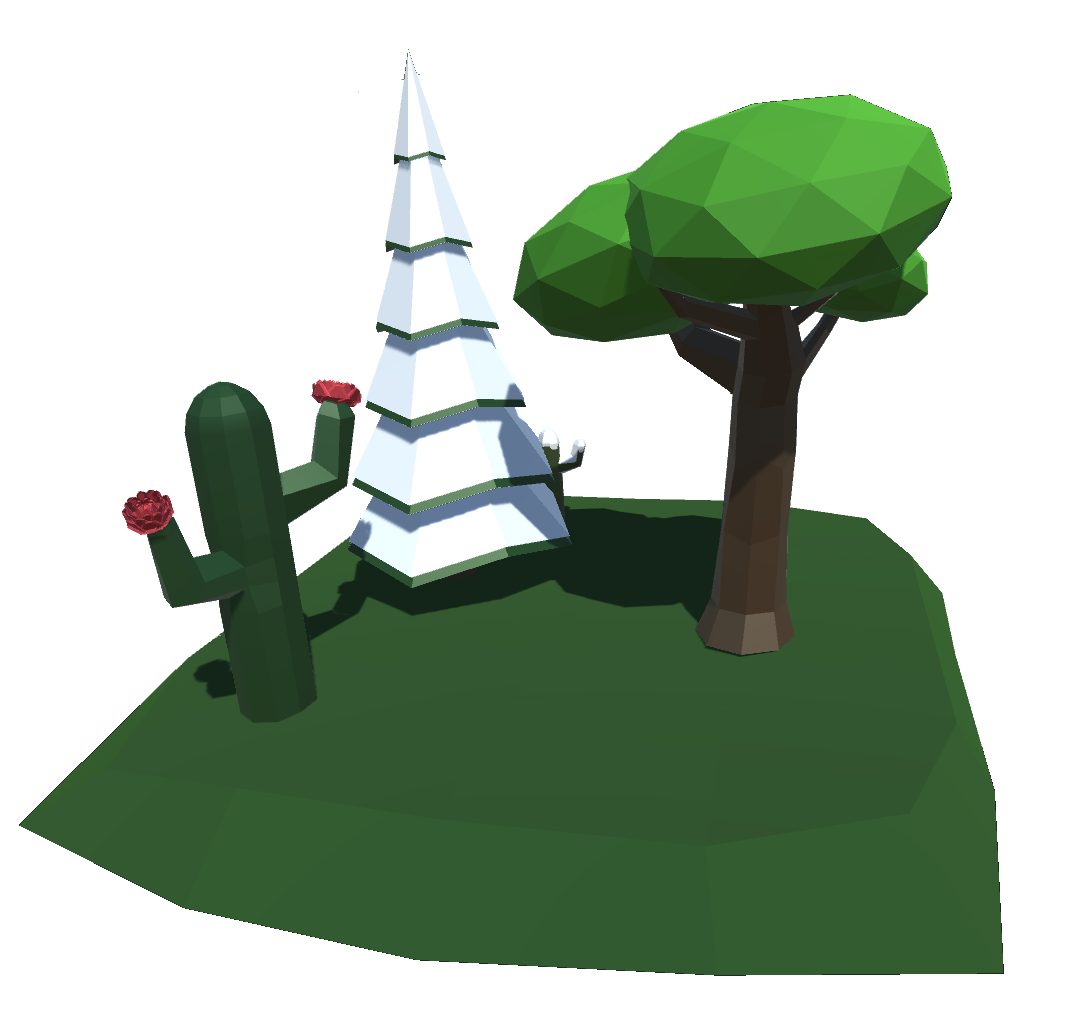
\includegraphics[width=10cm]{res/AeIcon.png}
\end{center} 
\begin{figure}[b]
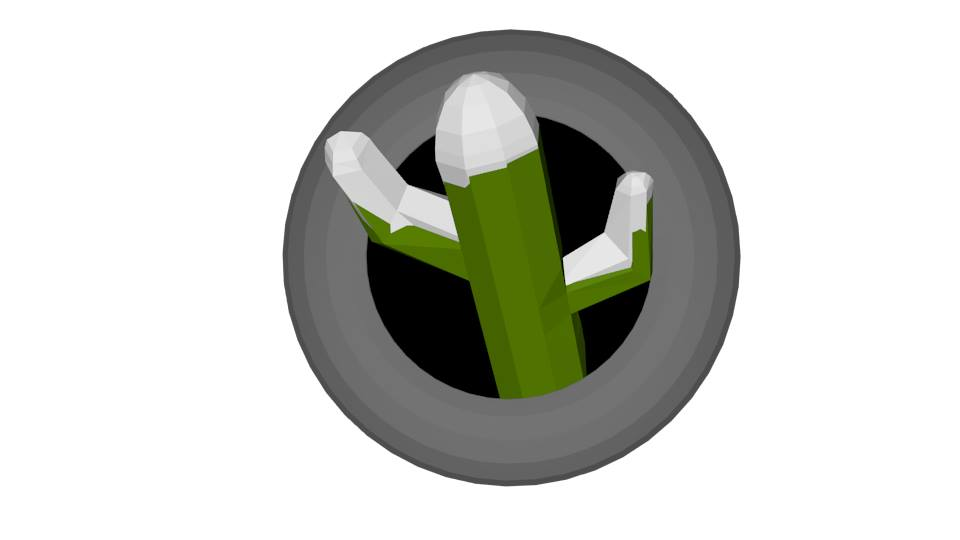
\includegraphics[height=2cm]{res/logo.jpg}
\hspace{10cm}

\includegraphics[height=2cm]{res/logo-epita-hd.png}
\end{figure}
\end{titlepage}


\pagebreak

\tableofcontents

\pagebreak

\section{Introduction}

Ceci est un manuel d'utilisation du jeu Aegina. Ce manuel raconte l'histoire du jeu Aegina et explique comment y jouer.

\section{Histoire}

Le monde d'Aegina est constitué d'une quasi infinité d'îles volantes se trouvant au-dessus d'un vide béant appelé les \textit{abysses}. Ce monde, contrairement au nôtre, est instable. Il ne partage pas nos lois de l'équilibre et de nombreux phénomènes étranges s'y produisent sans que l'on puisse les expliquer. La présence des \textit{abysses} n'est qu'un de ces phénomènes. Des cristaux, présents sur certaines îles, accentuent cette instabilité.

 Bien que ne vivant pas dans ce monde et n'ayant aucune information sur celui-ci, les êtres humains ont trouvé un moyen de \og téléporter \fg{} leurs déchets dans un néant qui n'est autre qu'Aegina. Lorsque les déchets arrivent directement dans les  \textit{abysses}, ils n'ont aucune influence sur la stabilité d'Aegina.  S'ils tombent sur une île, ils peuvent représenter un apport en ressource pour Aegina. L'aspect néfaste pour Aegina provient d'une sorte très particulière, presque barbare, de déchets.
 
 Certaines autorités humaines utilisent la \og téléportation \fg{} pour se débarrasser d'autres humains. Une fois dans le monde d'Aegina ceux-ci tentent désespérément de survivre. Ils finissent en général par arriver à activer des cristaux dont les pouvoirs quasi divins leur permettent d'échapper à la faim et à la mort. Certains ont alors voyagé d'île en île, créant quelques infrastructures telles que des ponts, laissant leur trace dans ce monde, mais l'amenant petit à petit à sa fin sans le savoir.
 
 Ille est le personnage que le joueur incarne dans Aegina. De père et de mère inconnus, Ille survit depuis son plus jeune âge seul dans une forêt. Bien que n'ayant pas d'amis, sauf si l'on peut considérer un écureuil comme un ami, Ille est très chaleureux et amical. Cependant, Ille n'est pas un enfant sauvage comme son histoire le laisse penser, il est légèrement civilisé et a lui-même choisi de vivre en ermite à cause de sa particularité. En effet, depuis sa petite enfance, Ille possède une force surhumaine (et un certain talent pour la construction). Il a lui-même construit sa maison à l'âge de neuf ans et est capable d'abattre des arbres comme un bucheron chevronné depuis qu'il sait manier une hache. Cependant, cette force effraie facilement les enfants de son âge et même les adultes, mais malgré tout Ille vit de façon paisible. Les repas de Ille ne sont pas très extravagants,  un jour cela peut être un sanglier et le lendemain un simple champignon. Une seule chose concernant sa nourriture lui importe, cette dernière doit être préparée car Ille tient toujours au fond de lui à se rapprocher des siens et l'action de préparer la nourriture lui donne l'impression d'être vraiment humain.
      
Son seul défaut, si l'on peut  considérer ceci comme un défaut, est d'être simplet. C'est d'une certaine façon une chance car c'est ce  qui à permis à l'aventure d'Aegina de commencer. 

Lors d'un hiver très rude, Ille n'eut pas d'autre choix que de voler de la nourriture dans un village avoisinant. Malheureusement, la discrétion n'étant pas son fort, il fut surpris en plein méfait et un garde tenta de l'arrêter. Ille essaya de passer le garde, mais il ne contrôla pas sa force et, en le bousculant, il le tua. Ille n'avait pas réalisé que le garde  était  extrêmement affaibli par le froid et la faim. Il fut alors poursuivi pour meurtre et rapidement arrêté car, malgré sa force, Ille restait humain. Il fut condamné à  mort et envoyé dans le néant qui n'était autre qu'Aegina. C'est à son réveil que le jeu commence.

Cependant, Ille n'est pas forcément seul en Aegina. Il pourra rencontrer d'autres personnes car la mort par envoi dans le néant est une pratique assez courante. Retrouver des amis dans ce monde dangereux peut être une bonne chose car dans Aegina le nombre de vos amis fait en partie votre force.


\pagebreak

\section{Comment jouer}
Controles : 
\begin{itemize}
\item \textbf{W}, \textbf{A}, \textbf{S}, \textbf{D} sont les touches permettant de se déplacer respectivement devant, a gauche, derrière et à droite.
\item la touche \textbf{C} permet de faire un bond en arrière
\item la touche \textbf{I} permet d'ouvrir et fermer l'iventaire
\item la touche \textbf{TAB} permet de voir tout les personnes connectés dans la partie 
\item la touche \textbf{MAJ} lorsqu'elle est associée à une touche de déplacement permet de courir 
\item le clique gauche de la souris permet de taper
\item le clique droit de la souris permet de taper lorsqu'un outil est equipé, ou d'interragir avec l'environnement lorsque aucun outils n'est équipé 

\end{itemize}

\pagebreak

\section{Menu principal}

\begin{figure}[h!]
\begin{center}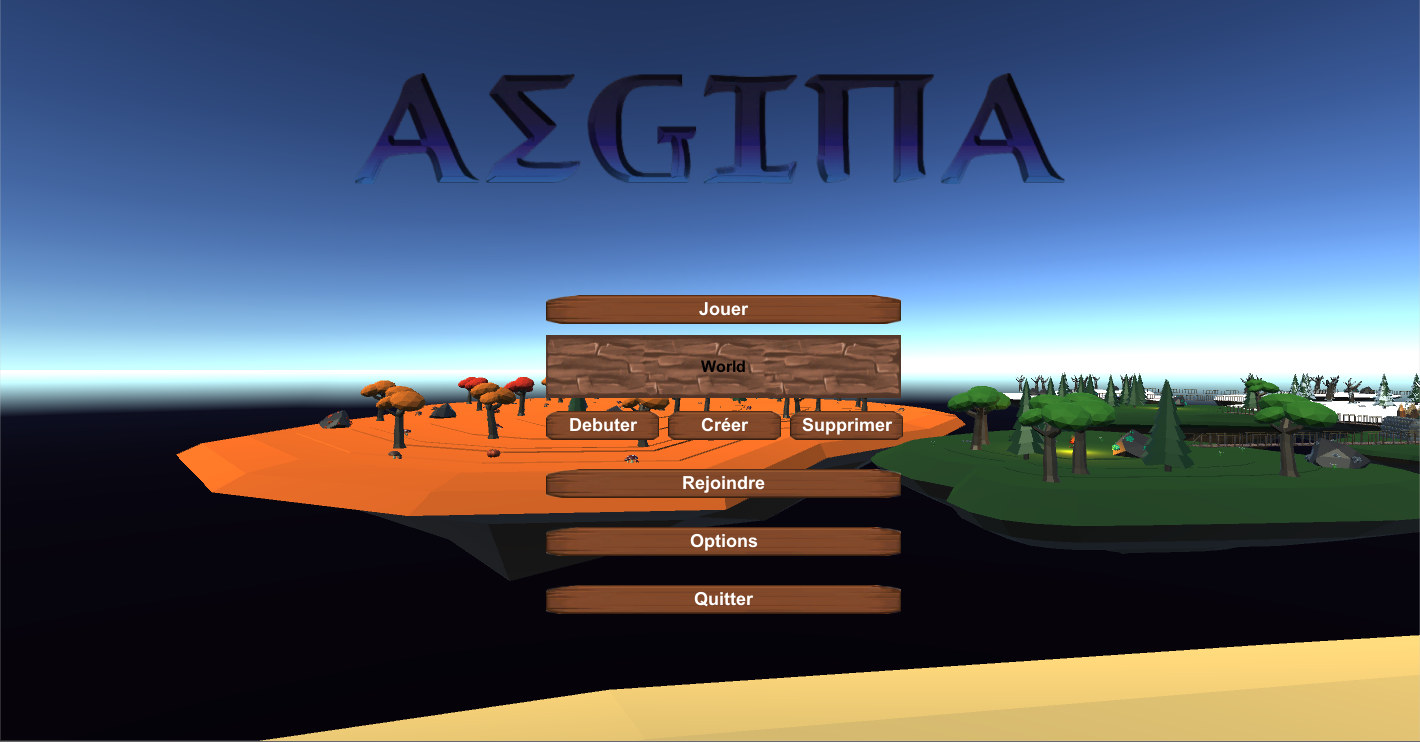
\includegraphics[width=10cm]{res/MenuPrincipal} % image à changer
\caption{Menu principal} 
\end{center}
\end{figure}

Le menu principal permet de choisir si l'on veut lancer un monde, Rejoindre un serveur, modifier des options ou quitter Le jeu.Si on veut créer un nouveau monde un nouvel interface apparaît

\begin{figure}[h!]
\begin{center}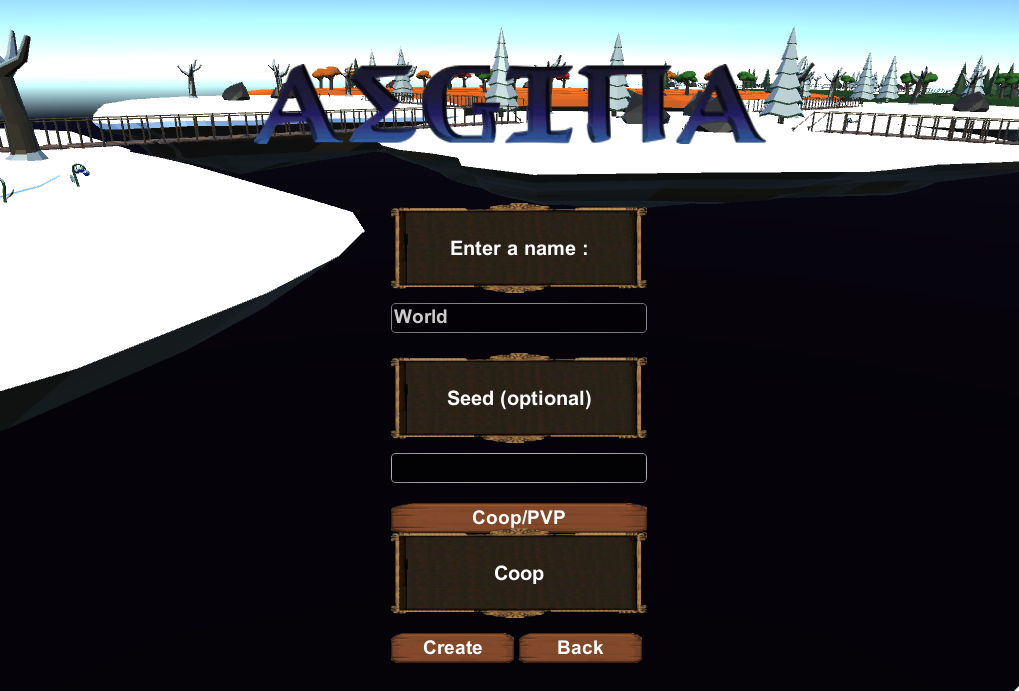
\includegraphics[width=10cm]{res/CreationMonde} % image à changer
\caption{Création de monde} 
\end{center}
\end{figure}

Losrque l'on cree un monde l'utilisateur peut choisir le nom du serveur qu'il veut creer. Il peut aussi choisir une graine afin de générer un monde spécifique à la graine. 

\begin{figure}[h!]
\begin{center}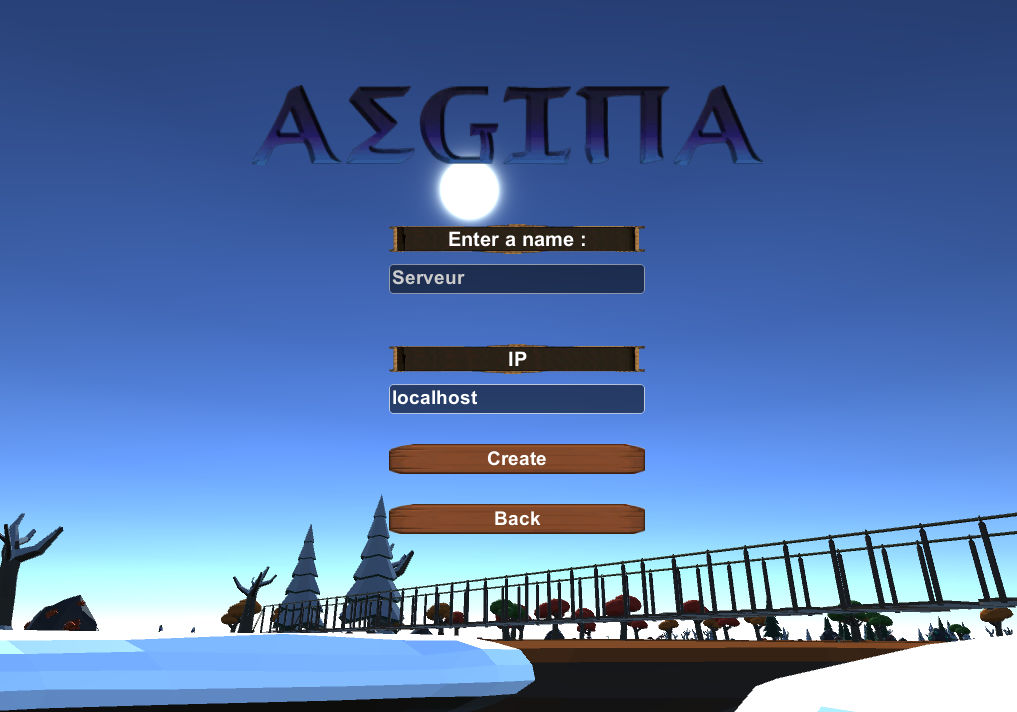
\includegraphics[width=10cm]{res/CreationServeur} % image à changer
\caption{Ajout de serveur} 
\end{center}
\end{figure}

Pour créer un serveur l'utilisateur doit lui donner un nom ainsi qu'une adresse ip

\begin{figure}[h!]
\begin{center}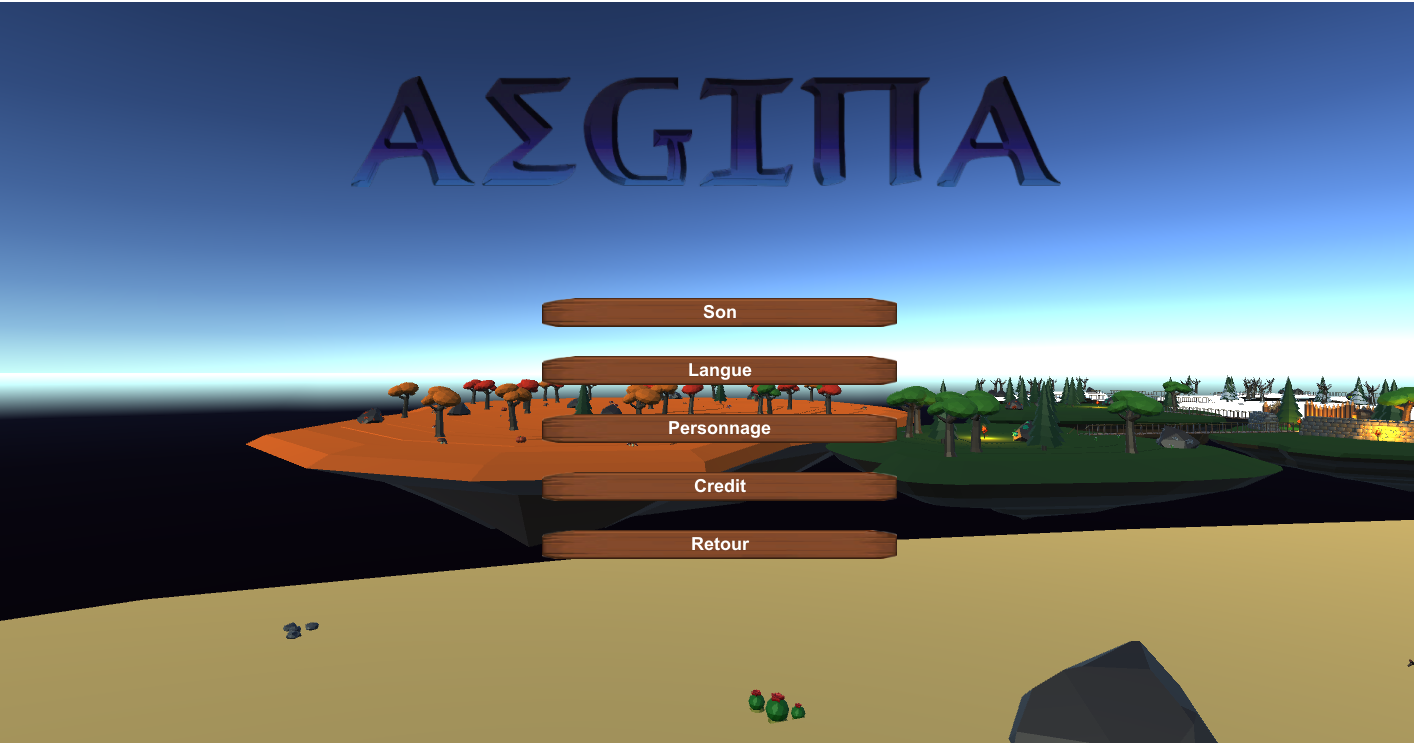
\includegraphics[width=10cm]{res/Options} % image à changer
\caption{Options} 
\end{center}
\end{figure}

Dans le menu d'option le joueur peut modifier la langue et le volume du son. En jeu il peut également changer la distance de rendu de la caméra.

\pagebreak

\begin{figure}[h!]
\begin{center}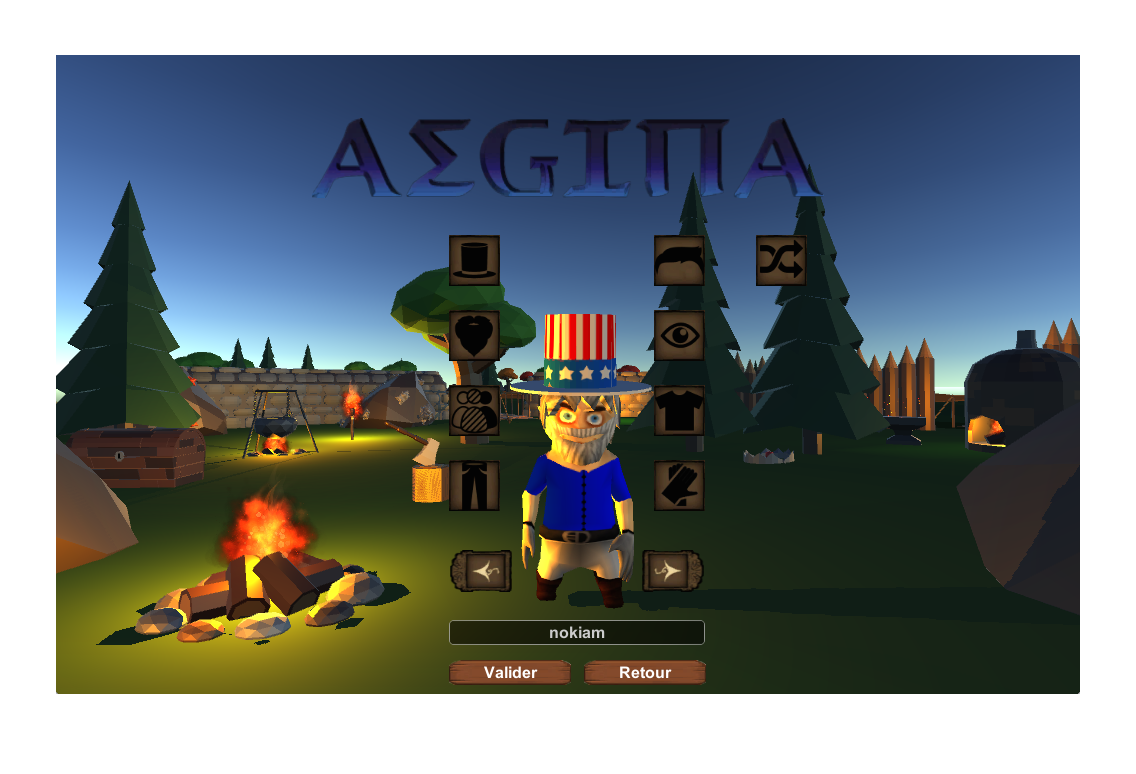
\includegraphics[width=10cm]{res/Personnalisation} % image à changer
\caption{Personnalisation du personnage} 
\end{center}
\end{figure}

Lors de la personnalisation de son personnage l'utilisateur possède un choix varié, afin de pouvoir créer le personnage aui lui correspond. Celui-si peut choisir parmis un ensemble de chapeux, barbes, yeux et habits afin de rendre son personnage unique.

\pagebreak

\section{Inventaire}


\begin{figure}[h!]
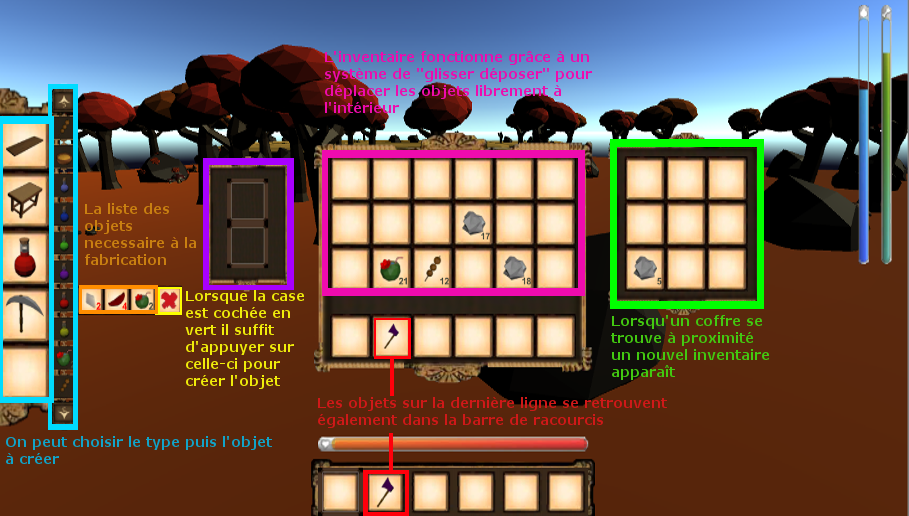
\includegraphics[width=15cm]{res/AideInventaire} % image à changer
\caption{Inventaire} 

\end{figure}

\pagebreak

\section{Cristaux}

\begin{figure}[h!]
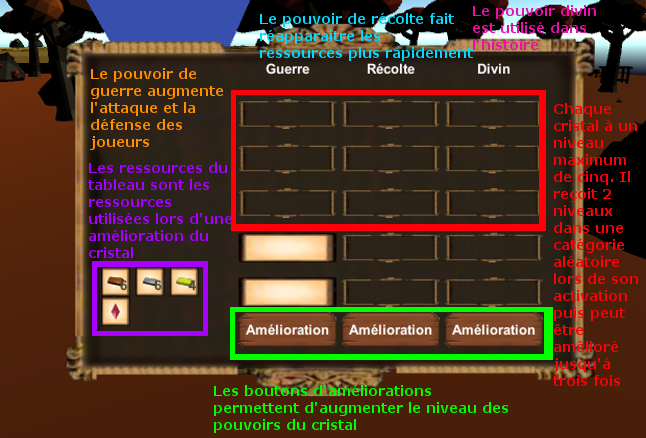
\includegraphics[width=15cm]{res/AideCristal} % image à changer
\caption{Interface des cristaux} 
\end{figure}

\pagebreak

\section{Cr\'{e}dit}
Concepteur :
\begin{itemize}
\item Romain MOUNIER
\item Julien MOUNIER
\item Florian AMSALLEM
\item Théo ISSARNI
\end{itemize}

Collaborateur : 
\begin{itemize}
\item Paul-Alexis MANDENGUE
\item Bastien LHUAIRE
\end{itemize}
\pagebreak

\section{Notes}

\end{document}
